\section{Peano's Natural Numbers}
\index{Peano}
It struck Giuseppe Peano in the early 1900's that tallies would be easier to get
right mathematically than digits. With the following two rules Peano introduced
the natural numbers to the formalism of math.
\begin{center}
\begin{minipage}{0.9\textwidth}
    \textit{
    $N_0$ vale ``numero'', et es nomen commune de 0,1,2, etc.\\
    $0$ $\to$  ``zero''\\
    $+$ $\to$ ``plus''.  Si $a$ es numero, $a+$ indica ``numero sequente $a$''.
    }
\end{minipage}
\end{center}
% It is fitting that the Italian is in italics.
(See G. Peano \emph{Formulaire de mathematiques.~I-V}, p.27.)
Replacing $+$ with \StrokeOne ~(and equating \StrokeFive$\defeq$\StrokeFour~\StrokeOne),
Peano's model of numbers is simply the grammar of tallies.

Today notation has evolved.  These numbers are now almost always designated as
\emph{natural numbers} and denoted $\mathbb{N}$.  Instead of $a+$ we now often
write $S~k$  or $S(k)$ calling it the ``successor'' to the natural number $k$.  
Programming however has held closer to the original with notation like 
\code{i++} and \code{++i}.

\index{tag}\index{\code{<name>}}\index{\code{::=}}\index{Walrus}
We mentioned Peano was merely recording the following grammar.  
% Today we write grammars with
% list of rules, called \emph{production rules}.  Some rules are to specify what
% makes up the alphabet of symbols in our grammar.  For Peano, $0$ and $S$ are the
% complete alphabet.  So we may write either $0$ on its own, or we may pre-pend
% the symbol $S$ to any existing natural number.  Each rule is given a name called
% a \emph{tag} and denoted \code{<tag-name>}. Since the Walrus
% $\defeq$ is our assignment, we use the
% ``Wowed Walrus'' $::=$ as assignment of production rules.   Taken together
% The grammar is the following. %, shown next to the childhood grammar for tallies.
\begin{center}
\begin{minipage}{0.5\textwidth}
\begin{Gcode}[]
<<Nat>> ::= 0 | S <Nat>
\end{Gcode}
\end{minipage}
% \hfill
% \begin{minipage}{0.45\textwidth}
% \begin{Gcode}[]
% <<Tally>> ::=  
% <<Tally>> ::= I <Tally>
% \end{Gcode}
% \end{minipage}
\end{center}
In the first rule we are told \code{0} is a natural number, denoted
\code{0:Nat}, just as any whitespace can start a tally. We say that the natural
number grammar \emph{accepts} \code{0} because it matched some production rule,
and the Tally grammar accepts whitespace, usually denoted $\epsilon$.  In the
second rule if we encounter an \code{S} it must be followed by an \emph{already
known} natural number.  So \code{S0:Nat} but \code{0S} would not be accepted as
it is not found as a production rule.  Going forward we use $\mathbb{N}$
for \code{Nat} and the usual name $0,1\defeq S0, 2\defeq SS0,\ldots$ as is common.
We retain the notation $n:\mathbb{N}$, instead of $n\in \mathbb{N}$, on account 
of the view that we shall later come to think of sets properly and us $\in$ notation 
when this happens.  


% \index{language}
% \begin{definition}
%     The \emph{words} (also called \emph{strings}) of letters accepted by a grammar is called
%     the grammar's \emph{language}.
% \end{definition}

% \begin{example}
% The natural numbers are the language of Peano's grammar, that is, the language of tallies.
% \end{example}


The significance of the ``already known'' clause of the rules is to prevent ambiguity 
with terms like $n=$\code{SSS....} where the \code{S} continue forever.
For if we remove one \code{S} form this $n$, the string is unchanged (thanks to 
the infinite number of $S$'s).  Since we are engaged in deciding if $n$ is a natural number and its substring 
is $n$, it is not of the form \code{S k} for \code{k:Nat}.  Hence the grammar 
rejects such an $n$.  Grammar's like these are called \emph{primitive recursive}
meaning that the recursion can only depend backwards 
in history.

\begin{definition}
    A production rule that appears more than once is called \emph{inductive}.
\end{definition}

\subsection{Drawing words in a grammar}
For each accepted word we can associate a graph where the nodes are the
production rule used at that stage to accept the fragment of the string, and
edges are any data needed by that rule to accept the substring.  This is called
the \emph{parse graph}.  In our cases they will always be trees so they are
often called \emph{parse trees}\index{parse tree} but you may also hear them
called \emph{abstract syntax trees} or ``ASTs''.\index{AST}\index{abstract
syntax tree}  In this example $0$ depends on nothing but $S$ depends on an
existing symbol.  Here are the first three parse trees in boxes.
\begin{center}
    \begin{tikzpicture}
    
    \node[draw] (A) at (0,0) {\begin{tikzpicture}
        \node (0) at (0,0) {0};
    \end{tikzpicture}};

    \node[draw] (B) at (3,0) {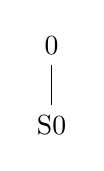
\begin{tikzpicture}
        \node (0) at (0,0) {0};
        \node (S0) at (0,-1) {S0};
        \draw[-] (0) -- (S0);
    \end{tikzpicture}};

    \node[draw] (C) at (6,0) {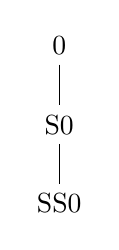
\begin{tikzpicture}
        \node (0) at (0,0) {0};
        \node (S0) at (0,-1) {S0};
        \node (SS0) at (0,-2) {SS0};
        \draw[-] (0) -- (S0);
        \draw[-] (S0) -- (SS0);
    \end{tikzpicture}};
    
    \draw[->] (A) edge["S"] (B);
    \draw[->] (B) edge["S"] (C);
    \draw[dashed,->] (C) edge["S"] (9,0);
\end{tikzpicture}
\end{center}
Between these boxes we have a different graph, the graph that 
plots how one production rule evolves an existing string to another.
This outside graph we call the \emph{word graph}.\index{word graph}  We often condense 
the parse trees to a string to draw the word graph compactly.
\begin{center}
    \begin{tikzpicture}
        \node (0) at (0,0) {0};
        \node (1) at (3,0) {S0};
        \node (2) at (6,0) {SS0};
        \coordinate (3) at (9,0);
        \draw[thick,->] (0) edge["S"] (1);
        \draw[thick,->] (1) edge["S"] (2);
        \draw[dashed,thick,->] (2) edge["S"] (3);
    \end{tikzpicture}
\end{center}

